% fig01 — four ways a rate can move
\documentclass[tikz,border=8pt]{standalone}

\usepackage[T1]{fontenc}
\usepackage{lmodern}
\usepackage{amsmath,amssymb,mathtools}
\usepackage{xcolor}

\usetikzlibrary{arrows.meta,positioning,fit,calc}

\definecolor{type1}{HTML}{0072B2}
\definecolor{type2}{HTML}{D55E00}
\definecolor{ink}{HTML}{1A1C1F}
\definecolor{inksoft}{HTML}{565B62}
\definecolor{rule}{HTML}{E3E6EA}
\definecolor{cardfill}{HTML}{F8FAFC}
\definecolor{type1fill}{HTML}{E9F1F8}
\definecolor{type2fill}{HTML}{FBEEE5}

\begin{document}
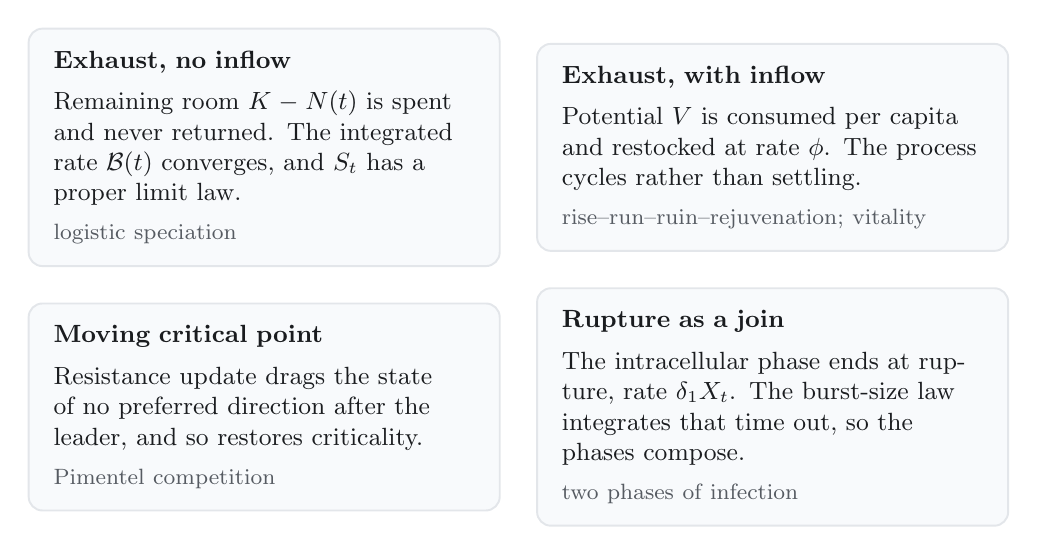
\begin{tikzpicture}[
    font=\small,
    card/.style={draw=rule, fill=cardfill, rounded corners=5pt,
                 line width=0.7pt, inner xsep=9pt, inner ysep=8pt,
                 text=ink, align=left, text width=5.35cm, minimum height=2.55cm},
  ]

\node[card] (a) at (0,0) {
  \textbf{Exhaust, no inflow}\\[4pt]
  Remaining room $K-N(t)$ is spent and never returned.
  The integrated rate $\mathcal{B}(t)$ converges, and $S_t$ has a proper limit law.\\[3pt]
  {\footnotesize\color{inksoft}logistic speciation}
};

\node[card, right=0.45cm of a] (b) {
  \textbf{Exhaust, with inflow}\\[4pt]
  Potential $V$ is consumed per capita and restocked at rate $\phi$.
  The process cycles rather than settling.\\[3pt]
  {\footnotesize\color{inksoft}rise--run--ruin--rejuvenation; vitality}
};

\node[card, below=0.45cm of a] (c) {
  \textbf{Moving critical point}\\[4pt]
  Resistance update drags the state of no preferred direction after the leader, and so restores criticality.\\[3pt]
  {\footnotesize\color{inksoft}Pimentel competition}
};

\node[card, below=0.45cm of b] (d) {
  \textbf{Rupture as a join}\\[4pt]
  The intracellular phase ends at rupture, rate $\delta_1 X_t$.
  The burst-size law integrates that time out, so the phases compose.\\[3pt]
  {\footnotesize\color{inksoft}two phases of infection}
};

\end{tikzpicture}
\end{document}
